%-------------------------------
%	PACKAGES AND OTHER DOCUMENT CONFIGURATIONS
%-------------------------------

% The \vref command specifies the location of the reference

\documentclass[
10pt, % Main document font size
a4paper, % Paper type, use 'letterpaper' for US Letter paper
oneside, % One page layout (no page indentation)
%twoside, % Two page layout (page indentation for binding and different headers)
headinclude,footinclude, % Extra spacing for the header and footer
BCOR5mm, % Binding correction
]{scrartcl}




%--------------------------------------------------------------
%	REQUIRED PACKAGES
%--------------------------------------------------------------

\usepackage[
nochapters, % Turn off chapters since this is an article        
beramono, % Use the Bera Mono font for monospaced text (\texttt)
%eulermath,% Use the Euler font for mathematics
pdfspacing, % Makes use of pdftex’ letter spacing capabilities via the microtype package
dottedtoc % Dotted lines leading to the page numbers in the table of contents
]{classicthesis} % The layout is based on the Classic Thesis style



\usepackage{arsclassica} % Modifies the Classic Thesis package
\usepackage[T1]{fontenc} % Use 8-bit encoding that has 256 glyphs
\usepackage[utf8]{inputenc} % Required for including letters with accents
\usepackage{libertinus} % The Libertinus font
%\usepackage[adobe-utopia]{mathdesign} % The Utopia font
\usepackage[czech]{babel} % Český jazyk
\usepackage{graphicx} % Required for including images
\graphicspath{{Figures/}} % Set the default folder for images
\usepackage{enumitem} % Required for manipulating the whitespace between and within lists
\usepackage{lipsum} % Used for inserting dummy 'Lorem ipsum' text into the template
\usepackage{subfig} % Required for creating figures with multiple parts (subfigures)
\usepackage{amsmath,amssymb,amsthm,amsfonts} % For including math equations, theorems, symbols, etc
\usepackage[czech]{varioref} % More descriptive referencing
\usepackage[top =3 cm, bottom = 3.5 cm, left = 1.5 cm, right = 1.5 cm]{geometry}
\usepackage{mathtools}
\usepackage{float}
\usepackage{caption}
\usepackage{color}
\usepackage{todonotes}

\usepackage{framed}

%------------------------------------------------------------
%	THEOREM STYLES
%------------------------------------------------------------

\theoremstyle{definition} % Define theorem styles here based on the definition style (used for definitions and examples)
\newtheorem{definition}{Definice}
\colorlet{shadecolor}{Red!15}
\newenvironment{Definition}
  {\begin{shaded}\begin{definition}}
  {\end{definition}\end{shaded}}


\theoremstyle{plain} % Define theorem styles here based on the plain style (used for theorems, lemmas, propositions)

\colorlet{shadecolor}{Blue!15}
\newtheorem{theorem}{Věta}
\newenvironment{Theorem}
    {\begin{shaded}\begin{theorem}}
    {\end{theorem}\end{shaded}}

\newtheorem{proposition}{Tvrzení}
\newenvironment{Proposition}
  {\begin{shaded}\begin{proposition}}
  {\end{proposition}\end{shaded}}

\newtheorem{lemma}{Lemma}
\newtheorem{corollary}{Důsledek}
\newtheorem*{corollary*}{Důsledek}

\theoremstyle{remark} % Define theorem styles here based on the remark style (used for remarks and notes)
\newtheorem{remark}{Poznámka}
\newtheorem{example}{Příklad}




%-------------------------------------------------------------
%	HYPERLINKS
%-------------------------------------------------------------

\hypersetup{
%draft, % Uncomment to remove all links (useful for printing in black and white)
colorlinks=true, breaklinks=true, bookmarks=true,bookmarksnumbered,
urlcolor=webbrown, linkcolor=RoyalBlue, citecolor=webgreen, % Link colors
pdftitle={}, % PDF title
pdfauthor={\textcopyright}, % PDF Author
pdfsubject={}, % PDF Subject
pdfkeywords={}, % PDF Keywords
pdfcreator={pdfLaTeX}, % PDF Creator
pdfproducer={LaTeX with hyperref and ClassicThesis} % PDF producer
}

 % Include the structure.tex file which specified the document structure and layout

%----------------------------------------------------
%	MATHEMATICS
%----------------------------------------------------

% Tělesa, obory íntegrity a metrické prostory
\newcommand{\C}{\mathbb{C}}
\newcommand{\R}{\mathbb{R}}
\newcommand{\N}{\mathbb{N}}
\newcommand{\Q}{\mathbb{Q}}
\newcommand{\Z}{\mathbb{Z}}
\renewcommand{\L}[2]{L^{#1} \left( #2 \right)} % Lebesgueovy prostory

\newcommand{\vc}[1]{\boldsymbol{#1}} % vektor
\newcommand{\mat}[1]{\mathbf{#1}} % matice

\newcommand{\norm}[1]{\left \Vert #1 \right \Vert} % norma vektoru
\newcommand{\set}[1]{ \left \lbrace #1 \right \rbrace} % množina
\newcommand{\const}{\mathrm{konst}} % konstanta

\newcommand{\F}{\mathcal{F} } % Fourierova transformace
\newcommand{\La}{\mathcal{L}} % Laplaceova transformace

% Označení funkcí
\newcommand{\Res}[2]{\mathrm{Res}_{#1} \, #2 \,} % residuum
\newcommand{\sgn}{\, \mathrm{sign} \,} % signum
\newcommand{\tg}{\,\mathrm{tg}\,} % možné značení tangens


%Značení derivací a integrálů
\newcommand{\der}[2]{\frac{\mathrm{d}#1}{\mathrm{d}#2}} % obyčejná derivace
\newcommand{\pder}[2]{\frac{\partial #1}{\partial #2}} % parciální derivace
\newcommand{\ppder}[3]{\frac{\partial^2 #1}{\partial #2 \partial #3}} % parciální derivace

\newcommand{\tder}[3]{\left( \pder{#1}{#2} \right)_{#3 = \const}} % termodynamická derivace

\newcommand{\fder}[2]{\frac{\delta #1}{\delta #2}} % funkcionální derivace
\newcommand{\ffder}[3]{\frac{\delta^2 #1}{\delta #2 \delta #3}} % funkcionální derivace

\newcommand{\D}{\mathrm{d} } % integrační znamení
\newcommand{\DD}{\mathrm{D}} % absolutní derivace
\newcommand{\intR}{\int_{-\infty}^{\infty}} % integrál přes reálnou osu



% Značení posloupností, limit a sum
\newcommand{\sequence}[2]{ \left \lbrace #1 \right \rbrace_{#2=1}^\infty} % posloupnost
\newcommand{\sumnorm}[1]{\sum_{#1}^\infty} 
\newcommand{\limplus}[1]{\lim_{#1 \rightarrow + \infty}}
\newcommand{\limminus}[1]{\lim_{#1 \rightarrow - \infty}}


%Značení distribucí
\newcommand{\dual}[2]{\left \langle #1 ,#2 \right \rangle} % dualita
\newcommand{\tf}[1]{\mathcal{D}(#1)} % prostor testovacích funkcí
\newcommand{\dis}[1]{\mathcal{D'}(#1)} % prostor distribucí
\newcommand{\Schwartz}[1]{\mathcal{S}(#1)} % Schwartzův prostor
\newcommand{\weakstar}{\rightharpoonup^*} % slabá* konvergence 
\newcommand{\supp}{\mathrm{supp}\,} % nosič funkcí % Include the mathematics.tex file which uses some mathematical operators

\hyphenation{Fortran hy-phen-ation} % Specify custom hyphenation points in words with dashes where you would like hyphenation to occur, or alternatively, don't put any dashes in a word to stop hyphenation altogether

%-------------------------------
%	TITLE AND AUTHOR(S)
%-------------------------------

\title{\normalfont\spacedallcaps{Article Title}} % The article title

%\subtitle{Subtitle} % Uncomment to display a subtitle

\author{\spacedlowsmallcaps{Miroslav Burýšek}} % The article author(s) - author affiliations need to be specified in the AUTHOR AFFILIATIONS block

\date{} % An optional date to appear under the author(s)




%-------------------------------------
%	TESTING
%-------------------------------------
% Load packages for testing

\usepackage{blindtext}
%\usepackage{showframe} % Uncomment to show boxes around the text area, margin, header and footer
\usepackage[inline]{showlabels}  \showlabels[\small\color{JungleGreen}]{}  % Uncomment to output the content of \label commands to the document where they are used


\begin{document}

%-------------------------------------------
%	HEADERS
%-------------------------------------------

\renewcommand{\sectionmark}[1]{\markright{\spacedlowsmallcaps{#1}}} % The header for all pages (oneside) or for even pages (twoside)
%\renewcommand{\subsectionmark}[1]{\markright{\thesubsection~#1}} % Uncomment when using the twoside option - this modifies the header on odd pages
\lehead{\mbox{\llap{\small\thepage\kern1em\color{halfgray} \vline}\color{halfgray}\hspace{0.5em}\rightmark\hfil}} % The header style

\pagestyle{scrheadings} % Enable the headers specified in this block





%-----------------------------------------
%	TABLE OF CONTENTS & LISTS OF FIGURES AND TABLES
%-----------------------------------------

%\maketitle % Print the title/author/date block

\setcounter{tocdepth}{2} % Set the depth of the table of contents to show sections and subsections only

%\tableofcontents % Print the table of contents

%\listoffigures % Print the list of figures

%\listoftables % Print the list of tables





%--------------------------------------
%	ABSTRACT
%--------------------------------------

%\section*{Abstract} 
% This section will not appear in the table of contents due to the star (\section*)


%---------------------------------------
%	AUTHOR AFFILIATIONS
%---------------------------------------

\let\thefootnote\relax\footnotetext{* \textbf{Kontakt:} \href{miroslav@burysek.eu}{miroslav@burysek.eu} }

%--------------------------------------

%\newpage % Start the article content on the second page,
% remove this if you have a longer abstract that goes onto the second page

%%----------------------------------------------------------------------------------------
%	INTRODUCTION
%----------------------------------------------------------------------------------------

\section{Introduction}

A statement requiring citation \cite{Figueredo:2009dg}.

%\lipsum[1-3] % Dummy text

Some mathematics in the text: $\cos\pi=-1$ and $\alpha$.
 
%----------------------------------------------------------------------------------------
%	METHODS
%----------------------------------------------------------------------------------------

\section{Methods}

\begin{align}
    \vc F(x,y,z;a,b,c) = xyz + \sum_{i=1}^N \dfrac{-b \pm \sqrt{b^2-4ac}}{2a} \label{eq:1}
\end{align}

%----------------------------------------------------------------------------------------
%	RESULTS AND DISCUSSION
%----------------------------------------------------------------------------------------

\section{Results and Discussion}

Reference to Figure~\vref{fig:gallery}. % The \vref command specifies the location of the reference

\begin{figure}[tb]
\centering 
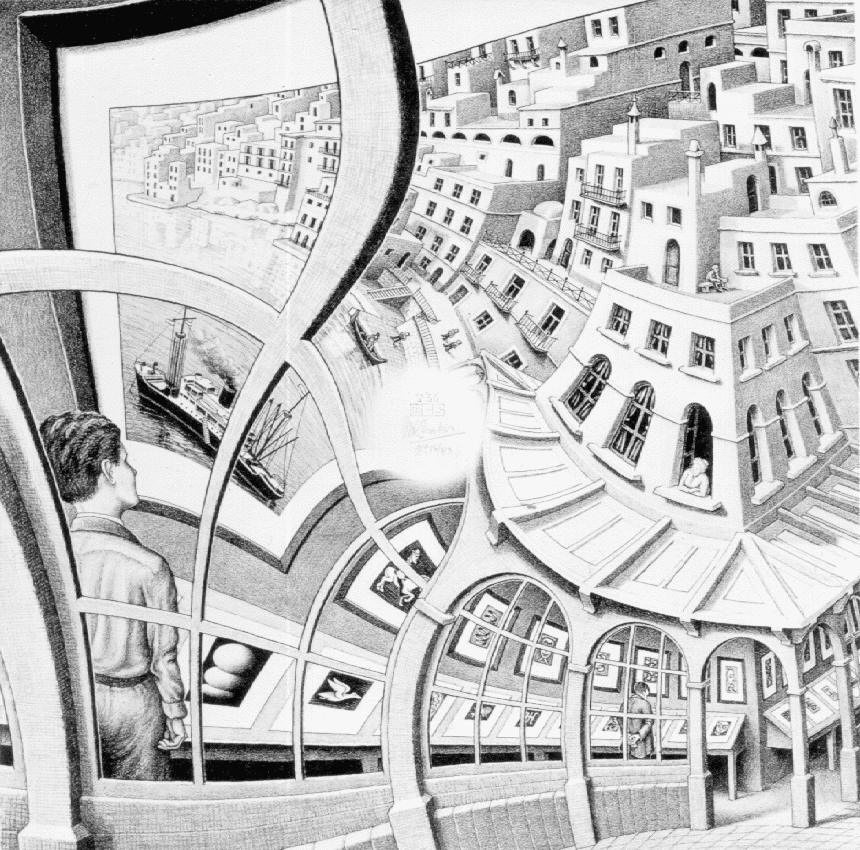
\includegraphics[width=0.5\columnwidth]{GalleriaStampe} 
\caption[An example of a floating figure]{An example of a floating figure (a reproduction from the \emph{Gallery of prints}, M.~Escher,\index{Escher, M.~C.} from \url{http://www.mcescher.com/}).} % The text in the square bracket is the caption for the list of figures while the text in the curly brackets is the figure caption
\label{fig:gallery} 
\end{figure}

\lipsum[10] % Dummy text

%------------------------------------------------

\subsection{Subsection}

\lipsum[11] % Dummy text

\subsubsection{Subsubsection}

\lipsum[12] % Dummy text

\begin{description}
\item[Word] Definition
\item[Concept] Explanation
\item[Idea] Text
\end{description}

\lipsum[12] % Dummy text

\begin{itemize}[noitemsep] % [noitemsep] removes whitespace between the items for a compact look
\item First item in a list
\item Second item in a list
\item Third item in a list
\end{itemize}



\lipsum[13] % Dummy text

Reference to Table~\vref{fig:ipsum}. 

%------------------------------------------------

\subsection{Figure Composed of Subfigures}

We use equation \eqref{eq:1} for counting the energy.

Reference the figure composed of multiple subfigures as Figure~\vref{fig:esempio}. Reference one of the subfigures as Figure~\vref{fig:ipsum}. % The \vref command specifies the location of the reference

\lipsum[15-18] % Dummy text

\begin{figure}[tb]
\centering
\subfloat[A city market.]{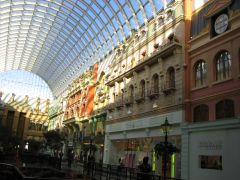
\includegraphics[width=.45\columnwidth]{Lorem}} \quad
\subfloat[Forest landscape.]{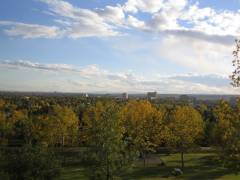
\includegraphics[width=.45\columnwidth]{Ipsum}\label{fig:ipsum}} \\
\subfloat[Mountain landscape.]{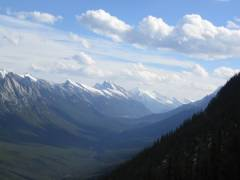
\includegraphics[width=.45\columnwidth]{Dolor}} \quad
\subfloat[A tile decoration.]{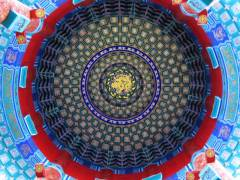
\includegraphics[width=.45\columnwidth]{Sit}}
\caption[A number of pictures.]{A number of pictures with no common theme.} % The text in the square bracket is the caption for the list of figures while the text in the curly brackets is the figure caption
\label{fig:esempio}
\end{figure}


%%-------------------------------------
%	BIBLIOGRAPHY
%-------------------------------------

\renewcommand{\refname}{\spacedlowsmallcaps{References}} % For modifying the bibliography heading

\bibliographystyle{unsrt}

\bibliography{sample.bib} % The file containing the bibliography

%------------------------------------

\section{Úvod}

\begin{definition}[Homogenní systém hydrodynamického typu]
    Homogenní systém hydrodynamického typu je systém parciálních diferenciálních rovnic tvaru
    \begin{align}
        \pder{u^i}{t} = f_j^{i \alpha} (u) \pder{u^j}{x^\alpha} \:, \quad 
        i = 1, \dots , N \:, \quad \alpha = 1, \dots , d \:.
    \end{align}
\end{definition}

\begin{proposition}[Transformace $f^{i \alpha}_j$] \label{prop:transformace-A} 
    Provedeme-li záměnu proměnných $u^i \mapsto v^a$ vztahem
    \begin{align}
        u^i = u^i(v^1,\cdots, v^N) \:,
    \end{align}
    pak se funkce $f^{i\alpha}_{j}$ transformují jako
    \begin{align}
        f^{a \alpha}_{b}(v) = \pder{v^a}{u^i} \pder{u^j}{v^b} f^{i \alpha}_j (u) \:.
    \end{align}
\end{proposition}
\begin{proof}
    Stačí rozepsat
    \begin{align}
        \pder{u^i}{t}(v) = \pder{u^i}{v^a} \pder{v^a}{t} \:, \\
        \pder{u^j}{x^\alpha}(v) = \pder{u^j}{v^b} \pder{v^b}{x^\alpha}\:,
    \end{align}
    takže
    \begin{align}
        \pder{u^i}{v^a} \pder{v^a}{t} = \pder{u^j}{v^b} f^{i \alpha}_j (v(u)) \pder{v^b}{x^\alpha}
    \end{align}
    a odtud
    \begin{align}
        \pder{v^a}{t} = \underbrace{\pder{v^a}{u^i} \pder{u^j}{v^b} f^{i \alpha}_j(v(u))}_{f^{a \alpha}_b(v)} \pder{v^b}{x^\alpha} \:.
    \end{align}
\end{proof}

Označme tedy $M^N$ prostor (varietu) s lokálními souřadnicemi $u^1,\cdots, u^N$. Pak lze na tvrzení \vref{prop:transformace-A} nahlížet jako na změnu souřadnic na $M^N$ a funkce $f^{i \alpha}_j$ jsou tenzory typu (1,1) pro každé zvolené $\alpha$. Pro případ, že $f^{i  \alpha}_j$ jsou ve speciálním tvaru, zavedeme bohatší geometrii na $M^N$ .

\begin{definition}
    \begin{enumerate}
        \item Poissonova závorka hydrodynamického typu funkcionálů $I_1$ a $I_2$ je definována vztahem
        \begin{align}
            \set{I_1,I_2} = \int \D x 
            \left[ \frac{\delta I_1}{\delta u^q(x)} f^{qp} \frac{\delta I_2}{\delta u^p(x)} \right] \:,
        \end{align}
        kde 
        \begin{align}
            A = (A^{qp}) = \left( g^{qp}(u) \der{}{x^\alpha} + b^{qp\alpha}_s(u) \pder{u^s}{x^\alpha} \right) \:,
        \end{align}
        přičemž $g^{ij \alpha}$ a $b_k^{ij \alpha}$ jsou dané funkce, $i,j,k = 1, \dots, N$ a $\alpha = 1, \dots, d $.

        Speciálně
        \begin{align}
            \set{u^i(x), u^j(y)} = g^{ij \alpha} [u(x)] \delta_\alpha(x-y) + b_k^{ij \alpha} [u(x)] u_\alpha^k(x) \delta(x-y) \:,
        \end{align}
        

        \item Hamiltonián hydrodynamického typu je definován vztahem
        \begin{align}
            H[u] = \int_{\R^d} h(u(x)) \D^d x \:,
        \end{align}
        kde $h[u]$ je nezávislá na $u_\alpha$, $u_{\alpha \beta}$. Funkci $h(u)$ nazýváme hamiltonovská hustota.

        \item Řekneme, že systém je hamiltonovský, jestliže lze psát
        \begin{align}
            u^i_t (x) = \set{u^i(x), H} := 
            \left[ g^{ij \alpha} [u(x)] \ppder{h(u)}{u^j}{u^k} + b_k^{ij \alpha} [u(x)] \pder{h(u)}{u^j} \right] u_\alpha^k(x) \:, \quad i = 1, \dots , d \:,
        \end{align}
        kde $H[u]$ je funkcionál hydrodynamického typu a $h$ je hamiltonovská hustota.
    \end{enumerate}
\end{definition}

\section{Jednodimenzionální případ}

Uvažujme nyní jednodimenzionální případ pro pevně zvolené $\alpha$. Zkoumáme tedy hamiltonovský systém
\begin{align}
    \pder{u^i}{t} (t,x) =&
    \left[ g^{ij} [u(t,x)] \ppder{h(u)}{u^j}{u^k} + b_k^{ij} [u(t,x)] \pder{h(u)}{u^j} \right] \pder{u^k}{x}(t,x) 
\end{align}
a Poissonova závorka hydrodynamického typu má tvar
\begin{align}
    \set{I_1,I_2} = \int \D x
    \left[ \frac{\delta I_1}{\delta u^q(x)} A^{qp} \frac{\delta I_2}{\delta u^p(x)} \right] \:, \quad A^{qp} = \left( g^{qp}(u) \der{}{x} + b^{qp}_s(u) \pder{u^s}{x} \right) \:,
\end{align}
speciálně
\begin{align}
    \set{u^i(x), u^j(y)} =& g^{ij} [u(t,x)] \delta'(x-y) + b_k^{ij} [u(t,x)] \pder{u^k}{x} \delta(x-y) \:. \label{eq:Poisson1D}
\end{align}

\begin{definition}
    Řekneme, že Poissonova závorka hydrodynamického typu je nedegenerovaná, jestliže $\det(g^{ij}) \neq 0$.
\end{definition}
Podle tvrzení \vref{prop:transoformace} níže je nedegenerovanost závorky invariantní vůči záměnně proměnných.

\begin{definition}
    Nechť je matice $(g^{ij}(u))$ nedegenerovaná. Definujme funkce $\Gamma^{i}_{jk}(u)$ vztahem
        \begin{align}
            b_k^{ij}(u) = -g^{is}(u) \Gamma^j_{sk}(u) \:, \quad i,j,k,s=1,\dots,N \:. \label{eq:definice-Gamma}
        \end{align}
\end{definition}

Dále uvidíme, že volba značení $g^{ij}$ a $\Gamma^{i}_{jk}$ není náhodná, ale že tyto funkce skutečně reprezentují metriku a složky afinní konexe na $M^N$. V důkazu mnoha tvrzení bude užitečný následující trik.

\begin{lemma}[O identitě s deltami] \label{lemma:delta}
    Platí
    \begin{align}
        f(y) \delta'(x-y) = f(x) \delta'(x-y) + f'(x) \delta(x-y) \:.
    \end{align}
\end{lemma}
\begin{proof}
    Přes distribuce.
    \begin{align*}
        \dual{f(x) \delta'(x-y)}{\psi(x)} 
        =& \dual{\delta'(x-y)}{f(x) \psi(x)} 
        = \\ =& -\dual{\delta(x-y)}{f'(x)\psi(x)} - \dual{\delta(x-y)}{f(x)\psi'(x)} 
        = \\ =& -f'(y) \psi(y) - f(y) \dual{\delta(x-y)}{\psi'(x)} 
        = \\ =& - \dual{f'(x)  \delta(x-y)}{\psi(x)} + f(y) \dual{\delta'(x-y)}{\psi(x)} 
        = \\ =& \dual{f(y) \delta(x-y) - f'(x) \delta'(x-y)}{\psi(x)} \:,
    \end{align*}
    odtud
    \begin{align}
        \dual{f(y) \delta'(x-y)}{\psi(x)} = \dual{f'(x) \delta(x-y)}{\psi(x)} + \dual{f(x) \delta'(x-y)}{\psi(x)} \:.
    \end{align} 
\end{proof}

\subsection{Geometrie prostoru $M^N$}

V tomto paragrafu si povšimneme, že na prostoru $M^N$ lze zavést tensorová pole a afinní konexi, což nám dále umožní formulovat tvrzení o ekvivalenci hamiltonovské a riemannovské struktury.

\begin{proposition}[O transformaci proměnných] \label{prop:transoformace}
    Uvažujme transformaci $u^i \mapsto v^i $  danou vztahem
    \begin{align}
        v^i = v^i (u^1, \dots, u^N) \:, \quad i = 1, \dots, N \:, \label{eq:transform}
    \end{align}
    která je diffeomorfismem třídy $C^2$.
    Pak platí následující tvrzení:
    \begin{enumerate}
        \item Poissonovy závorky se transformují jako tensory typu (2,0), tj.
        \begin{align}
            \set{v^p(u^i(x)),v^q(u^j(y))} = \pder{v^p}{u^i}(x) \pder{v^q}{u^j}(y) \set{u^i(x),u^j(y)} \:. \label{eq:transformace-zavorka}
        \end{align}
        \item Koeficienty $g^{ij}(u)$ se transformují jako tensory typu (0,2), tj.
        \begin{align}
            g^{pq}(v) = \pder{v^p}{u^i} \pder{v^q}{u^j} g^{ij}[u(v)] \:, \quad p, q = 1, \dots, N \:. \label{eq:transformace-metrika}
        \end{align}
        \item Koeficienty $\Gamma^i_{jk}$ se transformují jako Christoffelovy symboly (složky afinní konexe), tj.
        \begin{align}
            \Gamma^p_{qr} (v) = \pder{v^p}{u^i} \pder{u^j}{v^q} \pder{u^k}{v^r} \Gamma^i_{jk}(u) + \pder{v^p}{u^i} \ppder{u^i}{v^q}{v^r} \:. \label{eq:transformace-konexe}
        \end{align}
    \end{enumerate}
\end{proposition}

\begin{proof}
    \begin{enumerate}
        \item Přímým dosazením do definice
        \begin{align}
            \set{v^p(u^i(x)),v^q(u^j(y))} 
            =& \int \D x' \int \D y' \underbrace{\fder{v^p}{u^i(x')} }_{\pder{v^p}{u^i}(x') \delta(x-x')} \set{u^i(x'),u^j(y')} \underbrace{\fder{v^q}{u^j(y')} }_{\pder{v^q}{u^j}(y') \delta(y-y')}
            = \\ =& \pder{v^p}{u^i}(x) \pder{v^q}{u^j}(y) \set{u^i(x),u^j(y)} \:.
        \end{align}
        \item Rozepišme transformaci závorky \eqref{eq:transformace-zavorka} pomocí \eqref{eq:Poisson1D}
        \begin{align}
            g^{pq}[v(u(x))] \delta'(x-y) + b^{pq}_s[v(u(x))] \pder{v^s}{u^k}(x) \pder{u^k}{x} \delta(x-y)
            = \pder{v^p}{u^i}(x) \pder{v^q}{u^j}(y) \left[ g^{ij}[u(x)] \delta'(x-y) + b^{ij}_k[u(x)] \pder{u^k}{x} \delta(x-y) \right] \:. \label{eq:dosad}
        \end{align}
        V dalším pro přehlednost označme
        \begin{align}
            T^a_k(x) := \pder{v^a}{u^k}(x) \:.
        \end{align}
        Na pravé straně rovnice \eqref{eq:dosad} vyjádříme $T^q_j(y) \delta'(x-y)$ pomocí lemmatu \vref{lemma:delta}. Tím převedeme všechny funkce do proměnné $x$, což už dále nebudeme explicitně vypisovat. Dostaneme
        \begin{align}
            g^{pq}(v) \delta'(x-y) + b^{pq}_n(v) T^n_j \pder{u^j}{x} \delta(x-y) 
            = T^p_i T^q_j g^{ij}(u) \delta'(x-y) 
            + \left( \ppder{v^q}{u^j}{u^k} + T^p_i T^q_j b^{ij}_k \right) \pder{u^k}{x} \delta(x-y) \:.
        \end{align}
        Porovnáním členů s $\delta'$ dostaneme vztah pro transformaci metriky \eqref{eq:transformace-metrika}.
        \item Porovnáním členů s $\delta$ dostaneme
        \begin{align}
            b^{pq}_n(v) T^n_k =
            b^{ij}_k(u) T^p_i T^q_j + g^{ij}(u) T^p_i \ppder{v^q}{u^i}{u^k}
        \end{align}
        a po rozpisu pomocí \eqref{eq:definice-Gamma}
        \begin{align}
            - g^{ps}(v) \Gamma^{q}_{sn}(v) T^n_k =
            - g^{il}(u) \Gamma^j_{lk}(u) T^p_i T^q_j + g^{ij}(u) T^p_i \ppder{v^q}{u^i}{u^k} \:.
        \end{align}
        Na levé straně využijeme transformaci metriky \eqref{eq:transformace-metrika} a dostaneme
        \begin{align}
            -g^{ij}(u) \Gamma^q_{sm}(v) T^p_i T^s_j T^m_k = - g^{ij}(u) \Gamma^l_{jk} T^p_i T^q_l + g^{ij}(u) \ppder{v^q}{u^i}{u^k} T^p_i 
        \end{align}
        a po zkrácení $g^{ij}(u) T^p_i$
        \begin{align}
            \Gamma^l_{jk}(u) T^q_l = \Gamma^q_{sm}(v) T^s_j T^m_k + \ppder{v^q}{u^i}{u^k} \:.
        \end{align}
        V posledním kroku přenásobíme inverzní maticí $(T^{-1})^a_q$ a dostaneme
        \begin{align}
            \Gamma^a_{jk}(u) = \Gamma^q_{sm}(v) \pder{v^s}{u^j} \pder{v^m}{u^k} \pder{u^a}{v^q} + \ppder{v^q}{u^i}{u^k} \pder{u^a}{v^q} \:,
        \end{align}
        což je hledaný transformační vztah \eqref{eq:transformace-konexe}.
    \end{enumerate}
\end{proof}

\subsection{Ekvivalence riemannovské a poissonovské struktury}


\begin{theorem}[Ekvivalence pseudoriemannovské a hamiltonovské struktury] \label{theorem1:ekvivalence}
    Nechť $\det(g^{ij}) \neq 0$. Pak je vztahem \eqref{eq:Poisson1D} definována Poissonova závorka splňující antisymetrii, Leibnizovo pravidlo a Jacobiho identitu právě tehdy, když jsou splněny následující podmínky:
    \begin{enumerate}
        \item $g^{ij}$ je symetrický tensor, tj. definuje pseudo-riemannovskou metriku na prostoru $M^N$.
        \item Koeficienty $\Gamma^{i}_{jk}$ jsou složky Levi-Civitovy konexe příslušející metrice $g^{ij}$.
        \item Odpovídající konexe má nulovou torzi a křivost.
    \end{enumerate}
\end{theorem}

\begin{corollary*}
    Existují lokální souřadnice $w^i = w^i(u^1, \dots, u^N)$, $i = 1, \dots, N$ takové, že
    \begin{align}
        \tilde g^{ij}(w) = \const \:, \quad b^{ij}_k (w) = 0 \:.
    \end{align}
    V těchto souřadnicích je Poissonova závorka konstantní:
    \begin{align}
        \set{w^i(x),w^j(y)} = \tilde{g}^{ij} \delta'(x-y) \:.
    \end{align}
    Úplný lokální invariant Poissonových závorek je signatura pseudo-eukleidovské metriky $\tilde g^{ij}$.
    \todo[inline]{Co se tímhle myslí?}
\end{corollary*}

\begin{proof}[Důkaz věty \ref{theorem1:ekvivalence}]
    \textbf{Krok 1: Antisymetrie Poissonovy závorky implikuje symetrii metriky a kompatibilitu s $\Gamma^i_{jk}$}

    Poissonova závorka je antisymetrická, tj.
    \begin{align}
        \set{u^i(x),u^j(y)} + \set{u^j(y),u^i(x)} = 0 \:.
    \end{align}
    Rozepišme druhou závorku
    \begin{align}
        \set{u^j(y),u^i(x)} =  g^{ji}[u(y)] \delta'(y-x) + b^{ji}_k[u(y)] \pder{u^k}{y} \delta(y-x) \:.
    \end{align}
    Využijeme vztahů
    \begin{align}
        \delta(y-x) = \delta(x-y) \:, \quad \delta'(y-x) = -\delta'(x-y)
    \end{align}
    a lemmatu \vref{lemma:delta} aplikovaného na $g^{ji}[u(y)]\delta'(y-x)$. Dostaneme
    \begin{align}
        \set{u^j(y),u^i(x)} 
        = - g^{ji} [u(x)] \delta'(x-y) - \pder{g^{ji}}{u^k}[u(x)] \pder{u^k}{x} \delta(x-y) + b^{ji}_k[u(x)] \pder{u^k}{x} \delta(x-y)
        \:.
    \end{align}
    Celkově
    \begin{align}
        0 = \set{u^i(x),u^j(y)} + \set{u^j(y),u^i(x)} = \left[ g^{ij}[u(x)]  - g^{ji}[u(x)] \right] \delta'(x-y) + \left[ b^{ij}_k - \pder{g^{ji}}{u^k}  + b^{ji}_k  \right] \pder{u^k}{x} \delta(x-y) \:.
    \end{align}
    Výraz na pravé straně bude nulový právě tehdy, jestliže
    \begin{align}
        g^{ij} = g^{ji} \:, \label{eq:Th.Novikov-symetrie} \\
        \pder{g^{ij}}{u^k} = b^{ij}_k + b^{ji}_k  \:. \label{eq:Th.Novikov-konexe}
    \end{align}
    Rovnice \eqref{eq:Th.Novikov-symetrie} říká, že $g^{ij}$ je symetrický tenzor, dle předpokladu $\det g^{ij} \neq 0$ je nedegenerovaný, tj. definuje metriku na varietě $M^N$. Rovnice \eqref{eq:Th.Novikov-konexe} dává
    \begin{align}
        \pder{g^{ij}}{u^k} + g^{is} \Gamma_{sk}^j + g^{sj} \Gamma_{sk}^i = 0 \:,
    \end{align}
    takže $\Gamma_{ij}^k$ dává konexi kompatibilní s metrikou $g^{ij}$.


    \textbf{Krok 2: Jacobiho identita je ekvivalentní nulové torzi a křivosti} 
    
    Abychom dokázali, že je nulová křivost a torze, využijeme Jacobiho identity. Položme
    \begin{align}
        J^{ijk}(x,y,z) = \set{ \set{u^i(x),u^j(y)}, u^k(z) } + \set{ \set{u^j(y), u^k(z)}, u^i(x)} + \set{ \set{u^k(z), u^i(x)}, u^j(y)} \:.
    \end{align}
    Musíme ukázat, že je $J^{ijk}(x,y,z) = 0$ ve smyslu distribucí, tedy
    \begin{align}
        \dual{J^{ijk}(x,y,z)}{p_i(x)q_j(y)r_k(z)} = 0 \quad \text{pro } p_i, q_j, r_k \in \dis{R}
    \end{align}
    a protože se jedná o regulární distribuci, ověřujeme
    \begin{align}
        \int_{\R^{3}} J^{ijk}(x,y,z) p_i(x)q_j(y)r_k(z) \, \D x \D y \D z = 0\:.
    \end{align}
    Takový integrál lze převést na jednodimenzionální integrál
    \begin{align}
        \int_{\R} \sum_{\sigma, \tau =0}^2 A^{ijk}_{\sigma \tau} p_i q_j^{(\sigma)} r_k^{(\tau)} \, \D x = 0 \:,
    \end{align}
    kde koeficienty $A^{ijk}_{\sigma \tau}$ jsou nezávislé na $p,q,r$.
    Obdržíme tedy systém rovnic \begin{align}
        A^{ijk}_{\sigma \tau} = 0 \quad \forall i,j,k=1, \dots ,N \:; \quad 0 \leq \sigma, \tau \leq 2 \:.
    \end{align}\todo[inline]{Rád bych si funkce napsal explicitně, určitě se v nich objeví derivace druhého řádu někde? Ale nedaří se mi to sestavit.}

    Přepišme tyto rovnice explicitně. 
    Jedna z těchto rovnic dává
    \begin{align}
        A_{02}^{ijk} = b^{ij}_s g^{sk} - b^{kj}_s g^{si} = -g^{ip} \Gamma^{j}_{ps} g^{sk} + g^{km} \Gamma^{j}_{ms} g^{si} =0 \:,
    \end{align}
    odtud (po přenásobení $g_{ai}g_{bk}$)
    \begin{align}
        \Gamma^j_{ab} - \Gamma^j_{ba} = 0 \:.
    \end{align}
    Tento vztah říká, že jsou koeficienty afinní konexe symetrické, tj. příslušná konexe má nulovou torzi.

   Další z rovnic dává
    \begin{align}
        A_{00}^{ijk} = B^{ijk}_p(u) u^p_{xx} + C^{ijk}_{pq}(u) u^p_x u^q_x = 0 \:,
    \end{align}
    kde 
    \todo[inline]{Je v původním článku typo??}
    \begin{align}
        B^{ijk}_p 
        = (b^{jk}_{s,p} - b^{jk}_{p,s}) g^{si} + b_s^{ij} b_p^{sk} - b_s^{ik} b_p^{sj} \:.
    \end{align}
    Nulovost $B^{ijk}_p$ dává nulovou křivost, jak plyne z rozpisu
    \begin{align}
        B^{ijk}_p  
        =& -g^{is} \left( g^{jm}_{,p} \Gamma^k_{ms} + g^{jm} \Gamma^k_{ms,p} - g^{jm}_{,s} \Gamma^k_{mp} - g^{jm} \Gamma^k_{mp,s} \right) + g^{im} \Gamma^j_{ms} g^{sn} \Gamma^{k}_{np} - g^{im} \Gamma^k_{ms} g^{sn} \Gamma^j_{np}
        = \\ =& g^{is} g^{jn} \left( \Gamma^m_{np} \Gamma^k_{ms} - \Gamma^{m}_{ns} \Gamma^k_{mp} + \Gamma^{k}_{mp,s} -  \Gamma^{k}_{ms,p} \right) + g^{is} g^{nm} \left( \Gamma^j_{np} \Gamma^{k}_{ms} - \Gamma^j_{ns} \Gamma^k_{mp} \right) + g^{im} g^{sn} \left( \Gamma^j_{ms} \Gamma^k_{np} - \Gamma^k_{ms} \Gamma^j_{np} \right)
        = \\ =& -g^{is} g^{jn} \left( \Gamma^{m}_{ns} \Gamma^k_{mp}  - \Gamma^m_{np} \Gamma^k_{ms} + \Gamma^{k}_{ms,p} - \Gamma^{k}_{mp,s} \right)
        = \\ =& -g^{is} g^{jn} R^k_{nps} \:.
    \end{align}
    Takže křivost metriky $g^{ij}$ je nulová. Tím jsme dokázali, že pokud je vztahem \eqref{eq:Poisson1D} definována Poissonova závorka, jsou splněny podmínky 1-3.

    \textbf{Krok 3: Souřadnice, ve kterých je závorka triviální, dávají postačitelnost}

    Jestliže mají koeficienty afinní konexe $\Gamma_{ij}^k$ nulovou torzi i křivost, existují souřadnice $w^i=w^i(u^1,\dots,u^N)$ pro $i=1,\dots,N$ takové, že $g^{ij} = \const$ a $b^{ij}_k = 0$. V těchto souřadnicích je Poissonova závorka konstantní
    \begin{align}
        \set{w^i(x),w^j(y)} = \tilde{g}^{ij} \delta'(x-y) \:.
    \end{align}
    Jacobiho identita, antisymetrie i Leibnizovo pravidlo jsou pro tuto závorku triviálně splněny. Tím jsme ukázali postačitelnost podmínek (1)-(3) pro vlastnosti Poissonovy závorky.
\end{proof}

\subsection{Kdy je hydrodynamický systém hamiltonovský?}

Nyní můžeme explicitně přepsat podmínky, při kterých je obecný systém hydrodynamických rovnic hamiltonovský vůči nějaké nedegenerované Poissonově závorce. Nejprve si povšimneme, že funkce $f^i_j(u)$ lze přepsat pomocí Laplaceova–Beltramiho operátoru.

\begin{proposition}[O zápisu pomocí Laplaceova–Beltramiho operátoru]
    Mějme hamiltonovský systém rovnic
    \begin{align}
        \pder{u^i}{t} = f^i_k(u) \pder{u^k}{x} \:, \quad f^i_k(u) = g^{ij}(u) \ppder{h}{u^j}{u^k} - g^{is}(u) \Gamma^j_{sk}(u) \pder{h}{u^j} \:. \label{eq:hamiltonovsky-system}
    \end{align}
    Pak lze psát 
    \begin{align}
        f^i_k(u) = \nabla^i \nabla_k h(u) \:, 
    \end{align}
    kde $\nabla_j$ je Levi-Civitova kovariantní derivace metriky $g_{ij}$ a $\nabla^i = g^{is} \nabla_s$. 
\end{proposition}
\begin{proof}
    Přímým dosazením
    \begin{align}
        \nabla_k h(u) =& \pder{h}{u^k} \:, \\
        \nabla^i \nabla_k h(u) =& g^{is} \nabla_s \pder{h}{u^k} = g^{is} \left( \ppder{h}{u^s}{u^k} - \Gamma^j_{sk} \pder{h}{u^j} \right) = f^i_k(u) \:.
    \end{align}
\end{proof}

Pomocí tohoto zápisu snadno můžeme sepsat postačující podmínky hamiltonovskosti.
Důkaz plyne ihned z teorému \vref{theorem1:ekvivalence}.

\begin{theorem}[Postačující podmínka hamitonovskosti systému]
    Systém $u^i_t = f^i_j(u) u^j_x$ je hamiltonovský právě tehdy, když existuje nedegenerovaná metrika $g^{ij}(u)$, jejíž afinní konexe má nulovou křivost a splňuje
    \begin{align}
        g_{ij} f^k_j = g_{jk} f^k_i \:, \label{eq:gf=gf} \\
        \nabla_i f^k_j = \nabla_j f^k_i \label{eq:nablaf} \:.
    \end{align}
\end{theorem}

Speciálně vztah \eqref{eq:nablaf} říká, že $\nabla_i$ má nulovou torzi.


\subsection{Rekonstrukce metriky z $f^i_j(u)$?}

Máme-li zadaný hamiltonovský systém s maticí $f^i_j(u)$, lze metriku $g^{ij}(u)$ zkonstruovat jednoznačně? Tuto otázku nyní vyřešíme pro $N \geq 3$. 

Označme $\lambda_\alpha$ vlastní čísla matice $f^i_j(u)$. (Mohou být komplexní.) Předpokládejme, že jsou navzájem různá. Označme odpovídající bázi vlastních vektorů $e_\alpha(u)$. Definujme koeficient $c^\gamma_{\alpha \beta}(u)$ vztahem
\begin{align}
    [e_\alpha,e_\beta] = c^\gamma_{\alpha \beta} e_\gamma \:,
\end{align}
kde $[\cdot,\cdot]$ značí obyčejný komutátor funkcí. Předpokládejme dále, že pro navzájem různé $\alpha, \beta, \gamma$ je $c^\gamma_{\alpha \beta}$ různé od nuly .

\begin{definition}
    Matici $f^i_j(u)$ splňující podmínky výše nazveme hamiltonovskou maticí.
\end{definition}

\begin{theorem}[O rekonstrukci metriky]
    Nechť $N \geq 3$. Nechť je dána hamiltonovská matice $f^i_j(u)$. Pak lze zkonstruovat nedegenerovanou metriku $g^{ij}(u)$ s nulovou křivostí jednoznačně až na násobek konstantou.
\end{theorem}

\todo[inline]{Tomuhle nerozumím a myslím si, že v článku mají typo.}
\begin{proof}
    Z rovnice \eqref{eq:gf=gf} je vidět, že v bázi $e_\alpha$ je metrika $g^{ij}$ diagonální. 
    \todo[inline]{Opravdu?}
    V této bázi pak bude mít rovnice \eqref{eq:nablaf} tvar (zde se nesčítá přes opakované indexy)
    \begin{align}
        \partial_\alpha \lambda_\beta \delta_\beta^\gamma - \partial_\beta \lambda_\alpha \delta_\alpha^\gamma + (\Gamma_{\alpha \beta}^\gamma - \Gamma_{\beta \alpha}^\gamma ) \lambda_\gamma + \Gamma_{\beta \alpha}^\gamma (\lambda_\beta - \lambda_\alpha) = 0 \:.
    \end{align}
    Zde $\partial_\alpha$ je derivace ve směru $e_\alpha$ a konexe $\Gamma_{\alpha \beta}^\gamma$ jsou definované rovnostmi
    \begin{align}
        \nabla_{e_\beta} e_\alpha = \sum \Gamma^\gamma_{\alpha \beta} e_\gamma \:.
    \end{align}

    Normalizujme nyní vlastní vektory $e_\alpha$ tak, aby v této bázi byla metrika jednotková matice, tj. $g^{\alpha \beta} = \delta^{\alpha \beta}$.

    Výraz $c^\gamma_{\alpha \beta}$ má význam torze (z definice) a platí
    \begin{align}
        c^\gamma_{\beta \alpha} = \Gamma^\gamma_{\alpha \beta} - \Gamma^\gamma_{\beta \alpha} \:.
    \end{align} 

\end{proof}


\section{Vícerozměrný případ}

Ve vícerozměrném případě máme lineární bundle metrik a s nimi spojených konexí. Pro každou záměnu prostorových proměnných $x^\alpha \mapsto c^\alpha_\beta x^\beta$ pro $\alpha = 1, \cdots, d$ splňující $\det c^\alpha_\beta = 1$ se metrika $g^{ij \alpha}$ a konexe $b^{ij \alpha}_k$ transformují jako komponenty vektoru.

\begin{definition}
    Řekneme, že bundle metrik $g^{ij \alpha}$ je silně nedegenerovaný, jestliže pro nějakou sadu $c_\alpha$ je lineární kombinace $c_\alpha g^{ij \alpha}$ nedegenerovaná matice.
\end{definition}

\begin{theorem}
    Nechť je hamiltonovský systém silně nedegenerovaný.
    \begin{enumerate}
        \item Pro $N=1$ lze Poissonovu závorku redukovat na konstantní formu
        \begin{align}
            g^{ij}(u) = \tilde g^{ij}(u) \:.
        \end{align}

        \item Pro $N \geq 2$ lze Poissonovu závorku redukovat na lineární formu
        \begin{align}
            g^{ij \alpha}(u) = g^{ij \alpha}_k u^k + \tilde g^{ij \alpha} \:, \quad \alpha = 1, \cdots , d \:, \\
        \end{align}
        kde koeficienty $g^{ij \alpha}_k = b^{ij \alpha}_k + b^{ij \alpha}_k$, $\tilde g^{ij \alpha}$ a $b^{ij \alpha}_k$ jsou konstantní.
    \end{enumerate}
\end{theorem}


\end{document}